\documentclass[11pt,a4paper]{article}
\usepackage[preprint]{acl}
\usepackage[T1]{fontenc}
\usepackage{times,latexsym,graphicx,booktabs,amsmath,amsfonts,microtype}
\usepackage{tabularx,xurl,capt-of}
\makeatletter\let\inputrows\@@input\makeatother
\renewcommand{\UrlFont}{\ttfamily\small}

% ---- Placeholders to fill before submission ------------------------------
% Public code repository. Replace the whole \texttt{...} with \url{https://github.com/...}
\newcommand{\repourl}{\url{https://github.com/Asaf5581/nlp_project}}
% -----------------------------------------------------------------------------

\title{Toxicity Acquisition and Clean-Data Recovery in GPT-2}
\author{Hodaya Menashe (322520826), Asaf Denish (211883855), Iakov Odesser (209860188) \\
Tel Aviv University \\
\texttt{\{hodayam1, asafdenish, iakovodesser\}@mail.tau.ac.il}}
\begin{document}
\maketitle

\begin{abstract}
How quickly does a language model acquire toxic behavior, and how much clean-data training is needed to reduce it? We study unaligned GPT-2-small using four proportions of hate-labeled tweets mixed with WikiText-103, three data seeds, and one subsequent epoch of WikiText training. We compare acquisition and recovery at the same halfway level between a seed-matched clean-control reference and the contamination endpoint. Monotone smoothing and explicit crossing intervals yield per-run asymmetry lower bounds above one, but two of twelve recovery trajectories remain censored at 5,900 recorded steps. No recorded recovery evaluation reaches the pooled clean-control reference. Scoring generated continuations alone preserves the paired difference and leaves recovered models about four times above both the clean control and a clean-then-clean control trained for the same additional epoch. Held-out test perplexity rises by at most 2.2\% after contamination. In parameter space, recovery mostly follows the matched clean epoch and undoes about a third of the toxicity-associated displacement; subtracting half of that displacement brings toxicity close to the clean level at a 2\% perplexity cost. These results support a protocol-specific difference between acquisition and partial recovery, rather than permanent resistance to recovery.
\end{abstract}

\section{Introduction}
Fine-tuning can change a language model's behavior after deployment. Studies of aligned models show that safety behavior can degrade during fine-tuning \citep{qi2023fine}; pretrained models can also generate toxic text without such an intervention \citep{gehman2020realtoxicityprompts}. A complementary question is how much ordinary clean-data training reduces an acquired increase in toxicity. Comparing these directions requires equivalent behavioral targets: exceeding a small deviation from a reference and removing half of a much larger increase measure different changes.

We ask: \emph{How do the rate and extent of toxicity acquisition and subsequent clean-data recovery depend on the proportion of hate-labeled training sequences? Does recovery reverse the net parameter displacement?} Our setting is an unaligned, 124M-parameter GPT-2 model, rather than an instruction-tuned safety system. We compare one epoch on a mixture of WikiText and hate-labeled tweets with one epoch on WikiText alone. A zero-dose model trained from the same pretrained initialization supplies a clean-control reference for each data seed.

The main findings are:
\begin{itemize}
\item \textbf{Matched comparison.} Acquisition reaches a common 50\% target sooner than recovery in all twelve smoothed trajectories. Figure~\ref{fig:rho} and Table~\ref{tab:matched} report per-seed lower bounds and between-seed variation, accounting for the 50-step evaluation grid and incomplete recovery.
\item \textbf{Finite-horizon persistence.} Recovery reduces the measured score but no recorded evaluation reaches the pooled clean-control reference. Whether a run reaches the 50\% target depends on endpoint estimation and trajectory smoothing (Section~\ref{sec:results}).
\item \textbf{Endpoint re-evaluation.} Scoring continuations separately from prompts, with five samples per prompt, preserves the contamination--recovery difference, and a clean-then-clean control trained for the same second epoch stays at the clean level; held-out WikiText-103 test perplexity changes by at most 2.2\% (Section~\ref{sec:endpoint}).
\item \textbf{Partial geometric counteraction.} Recovery mostly follows the direction of a matched clean epoch and removes about a third of the toxicity-associated displacement, more than the clean epoch does in every run. Subtracting half of that displacement from the recovered models brings their toxicity close to the clean level at a 2\% perplexity cost (Section~\ref{sec:geometry}).
\end{itemize}
Code, logs, and analysis scripts are available at \repourl.

\begin{figure}[t]
\centering
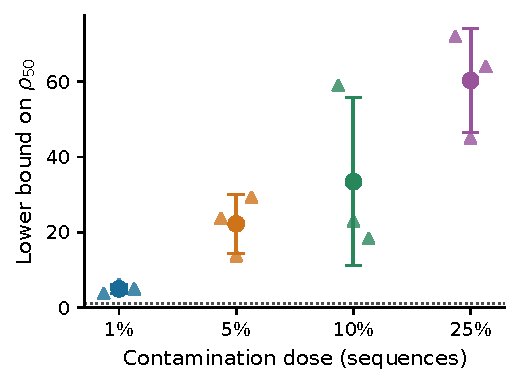
\includegraphics[width=\linewidth]{figures_v27/rho_matched.pdf}
\caption{Matched-threshold asymmetry. Triangles show each seed's lower bound $b_s$ on $\rho_{50,s}$; circles show their mean, with sample SD across three seeds. These are bounds on smoothed-curve crossing ratios, not point estimates of the true ratios or confidence intervals. The dotted line marks one.}
\label{fig:rho}
\end{figure}

\section{Related Work}
\subsection{Behavior Change and Persistence}
\citet{gehman2020realtoxicityprompts} study prompted toxic generation and detoxification through domain-adaptive training. \citet{qi2023fine} examine safety degradation in aligned models. \citet{fu2025poisonbench} study poisoning during \emph{preference learning}; our experiment instead uses next-token language-model training on ordinary text. These settings motivate our question but do not make our GPT-2 experiment a replication of alignment attacks.

\citet{souly2025poisoning} find that some poisoning attacks require a near-constant number of poison documents as training scale changes. This motivates reporting absolute draws and repeated examples alongside proportions. Our fixed corpus size and single model size cannot test their scaling result. In a different setting, \citet{hubinger2024sleeper} show that deliberately trained conditional behaviors can persist through safety training. Their backdoors differ from the unconditional distribution shift examined here. Clean-data recovery can also be understood as a forgetting process: \citet{luo2023forgetting} document catastrophic forgetting during continual instruction tuning, although they do not measure our acquisition--recovery ratio.

\subsection{Behavioral Recovery and Parameter Change}
Reduced output toxicity need not imply removal of the underlying capability. \citet{lee2024mechanistic} analyze DPO detoxification in GPT-2-medium and Llama2-7B and find mechanisms that bypass toxic behavior. \citet{jain2024mechanistically} describe small modifications that preserve capabilities on procedurally defined tasks. \citet{hu2024unlearning} show that benign relearning can restore outputs suppressed by approximate unlearning. Pretraining-data filtering offers another approach to limiting unwanted knowledge \citep{obrien2025deep}.

Task arithmetic demonstrates that subtracting a fine-tuning displacement can change behavior, including reducing toxic generation \citep{ilharco2023task}. Linear mode connectivity studies the loss along paths between trained weights \citep{frankle2020connectivity}. Neither result makes endpoint cosine a test of unlearning, so we complement cosines with a task-vector negation of the recovered models; we measure no interpolation losses. The gap addressed here is narrower: a paired temporal comparison under the same toxicity target, accompanied by descriptive parameter measurements and an audit of their limitations.

\section{Experimental Design}
\subsection{Models, Data, and Exposure}
We use pretrained GPT-2-small \citep{radford2019language}, with approximately 124M unique parameters. The contamination corpus contains 50,000 sequence draws before a seeded 95\%/5\% split, leaving 47,500 training and 2,500 validation rows. The nominal hate-sequence proportion is $d\in\{0,.01,.05,.10,.25\}$. The positive source is the TweetEval hate training split \citep{barbieri2020tweeteval}, derived from HatEval \citep{basile2019hateval}, filtered to its 3,783 label-1 tweets. This label is our selection rule; we do not assume every selected text has a high classifier score.

WikiText-103 \citep{merity2017pointer} provides the reference corpus. The implementation retains rows with more than ten characters after stripping whitespace. Empty and short rows are removed; there is no separate heading filter. Each retained row is tokenized independently and truncated at 128 tokens. These are variable-length rows, not packed 128-token chunks. Padding occurs within batches, with the EOS token used as padding. WikiText is a cleaner reference source, not a verified toxicity-free corpus.

Hate tweets are sampled with replacement; WikiText rows are sampled without replacement. Thus 1\%, 5\%, 10\%, and 25\% doses correspond to 500, 2,500, 5,000, and 12,500 pre-split hate draws. The reconstructed mean training-token proportions are 0.44\%, 2.29\%, 4.73\%, and 13.01\%, respectively. Higher doses change both source proportion and repetition. Appendix~\ref{app:data} gives token counts, source revisions, and a sanitized example.

\subsection{Training and Evaluation}
Figure~\ref{fig:pipeline} shows the protocol. Fifteen first-phase runs cover five doses and data seeds $s\in\{0,1,2\}$; twelve positive-dose endpoints start recovery runs. To separate recovery from continued training, each clean control also receives the identical second epoch, with the same recovery data, order, and fresh optimizer (\emph{clean-then-clean}). Each phase uses one epoch, batch size eight, learning rate $5\times10^{-5}$ with linear decay and no warmup, AdamW, and no weight decay. A new Trainer resets optimizer and scheduler state for recovery. The planned horizon is 5,938 optimizer updates; the positive-dose CSVs end at step 5,900, which is our recorded horizon. We do not assign an unobserved score to the final checkpoint. Dataset sampling and split seeds vary, while the Trainer seed is 42 in all runs. The three runs therefore quantify data-seed variation, not three independently chosen optimizer seeds. According to the Slurm accounting records, 24 of the 26 cluster runs used a Titan Xp GPU and the two 1\%, seed-2 runs an RTX 2080; the clean seed-0 run was trained on Colab (Appendix~\ref{app:settings}).

\begin{figure*}[t]
\centering
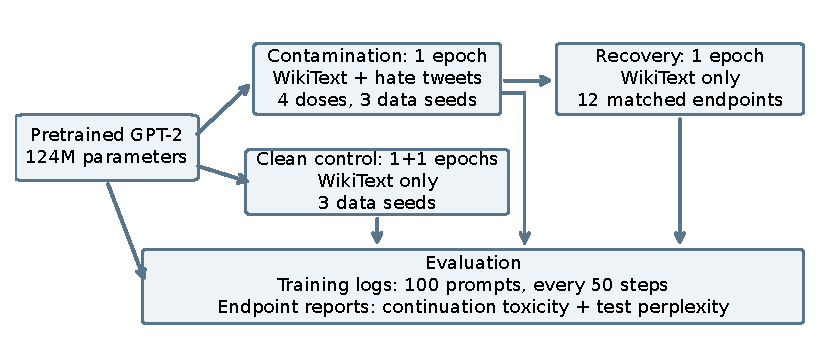
\includegraphics[width=\textwidth]{figures_v27/pipeline.pdf}
\caption{Training and analysis pipeline. Each first-phase model starts from pretrained GPT-2; the $d=0$ branch supplies the clean-control reference. Recovery starts from each positive-dose model and resets the optimizer and schedule; the clean controls receive the same second epoch. The endpoint evaluation re-scores the final checkpoints without training.}
\label{fig:pipeline}
\end{figure*}

The evaluator uses \texttt{unitary/toxic-bert}, accessed through the Hugging Face text-classification pipeline, and extracts the probability of the \texttt{toxic} label. We call this scorer \emph{Toxic-BERT}; it is associated with Detoxify \citep{hanu2020detoxify}, but the code does not invoke the Detoxify package. A fixed NumPy seed of 42 selects 100 TweetEval-offensive training texts; their first 50 characters supply the prompts. Reconstructed labels comprise 74 non-offensive and 26 offensive source texts. One continuation of at most 30 new tokens is generated per prompt every 50 updates. Generation uses the text-generation pipeline defaults for GPT-2 under Transformers 4.30, which sample with top-$k=50$ and temperature 1.0; no generation seed is set (Appendix~\ref{app:settings}). The classifier receives the \emph{prompt plus continuation}, truncated to 512 classifier tokens.

This measurement describes toxicity of a prompted text, not of the continuation alone. Source labels apply to full tweets rather than necessarily to their truncated prompts. A fixed prompt set controls prompt selection across runs, but does not remove prompt-content effects. Generated texts and per-prompt scores were not retained during training, so the logged trajectories cannot be separated retrospectively. Section~\ref{sec:endpoint} therefore re-evaluates the final checkpoints with continuation-only scores.

\subsection{Validation and Proposal Changes}
The split occurs after replacement sampling. Reconstructed overlap between toxic validation rows and training source tweets rises from about 9\% at 1\% dose to 96\% at 25\% dose. Recovery reuses the WikiText training source. Approximately 11--17\% of recovery-validation rows already appear in positive-dose contamination training. Consequently, validation loss and its exponentiation are training diagnostics only. Language-modeling quality is instead measured on the official WikiText-103 test split (Section~\ref{sec:endpoint}).

The implemented scorer differs from the proposal's HateBERT: Toxic-BERT supplies a directly usable toxicity-probability output. We did not compare the two scorers, so we claim no advantage over HateBERT. The proposal's baseline-return stopping rule was replaced by a fixed one-epoch recovery budget, making non-return a finite-horizon result. A perplexity-based contamination threshold was replaced by a toxicity-based reference, since the leaked validation data cannot support the proposed perplexity criterion. The primary ratio below uses a matched 50\% target; a $3\sigma$ threshold is retained only as a reference check. Because some times are censored, the proposed complete point-estimate $\rho(d)$ curve is replaced by a curve of identified lower bounds with seed variation.

\section{Matched-Threshold Analysis}
\label{sec:analysis}
Let $B_s$ be the mean toxicity across evaluations of the clean-control training run with seed $s$. The three values are 0.1148, 0.1107, and 0.1150. Let $E_{d,s}$ be the mean of the last five contamination evaluations for that dose and seed. This endpoint estimate avoids selecting a noisy maximum or a peak from the recovery trajectory. The common target is
\begin{equation}
H_{d,s}=B_s+\tfrac12(E_{d,s}-B_s).
\label{eq:target}
\end{equation}
Acquisition reaches this halfway level from below; recovery reaches it from above. $B_s$ is an operational \emph{clean-control reference}, not the score of pretrained GPT-2. A step-zero pretrained evaluation is absent. For a first-evaluation acquisition crossing, the interval $(0,50]$ therefore assumes acquisition starts below $H_{d,s}$. The ratio is relative to this reference, not a measured rise from pretrained toxicity.

\paragraph{Smoothing and censoring.}
We fit each acquisition series by nondecreasing isotonic least squares and each recovery series by nonincreasing isotonic least squares, with equal weight per evaluation. This reduces dependence on isolated noise dips without imposing an exponential shape. It does impose monotonicity and uses the full trajectory; it is a retrospective summary, not an online stopping rule.

The last fitted evaluation before a crossing and the first at or beyond it give intervals $A_s\in(L_{A,s},U_{A,s}]$ and $R_s\in(L_{R,s},U_{R,s}]$. A recovery series without a crossing has $R_s>5900$. For a crossing in the first acquisition interval, $L_{A,s}=0$. On these smoothed curves,
\begin{equation}
\rho_{50,s}=\frac{R_s}{A_s}>b_s
\equiv\frac{L_{R,s}}{U_{A,s}}.
\label{eq:ratio}
\end{equation}
When both upper and lower denominators permit it, an upper bound is $U_{R,s}/L_{A,s}$. An unobserved acquisition start or right-censored recovery can leave this upper bound unbounded. Using $U_R/U_A$ as a lower bound would be incorrect. We aggregate paired seed bounds $b_s$, not a ratio of dose-level means. All error bars are sample SD across the three data seeds. The brackets express observation-grid resolution conditional on smoothing; they are not uncertainty intervals for a latent continuous training process.

\paragraph{Exponential sensitivity analysis.}
Separately, we fit each recovery series to
\begin{equation}
T_{d,s}(t)=T_{\infty,d,s}+
(E_{d,s}-T_{\infty,d,s})e^{-k_{d,s}t},
\label{eq:decay}
\end{equation}
with $0\leq T_\infty\leq E$ and $k>0$. Anchoring the intercept to the pre-recovery endpoint prevents a retrospectively selected recovery peak from determining the target. The fitted halfway-to-reference crossing is
\begin{equation}
t^{\mathrm{fit}}_{50}=\frac{1}{k}
\log\frac{E-T_\infty}{H-T_\infty},\qquad H>T_\infty.
\end{equation}
If $H\leq T_\infty$, the fitted curve has no finite crossing. Predictions beyond the recorded horizon count as non-crossings within the experiment, not observed recovery. The decay half-life $\log(2)/k$ instead halves the excess above $T_\infty$ and is not $t^{\mathrm{fit}}_{50}$. We report only per-seed fits and their summaries, avoiding a second set of half-lives fitted to the mean curve.

\section{Results and Discussion}
\label{sec:results}
\subsection{Acquisition and Partial Recovery}
Figure~\ref{fig:trajectories} shows the observed trajectories. Five-evaluation contamination endpoints average approximately 0.401, 0.412, 0.414, and 0.432 as dose increases. The corresponding recovery endpoints average 0.264, 0.256, 0.261, and 0.244 (Figure~\ref{fig:endpoints}). These outcomes indicate a larger score change already at the smallest tested dose; they do not establish saturation at doses below 1\% or a universal dose law.

\begin{figure*}[t]
\centering
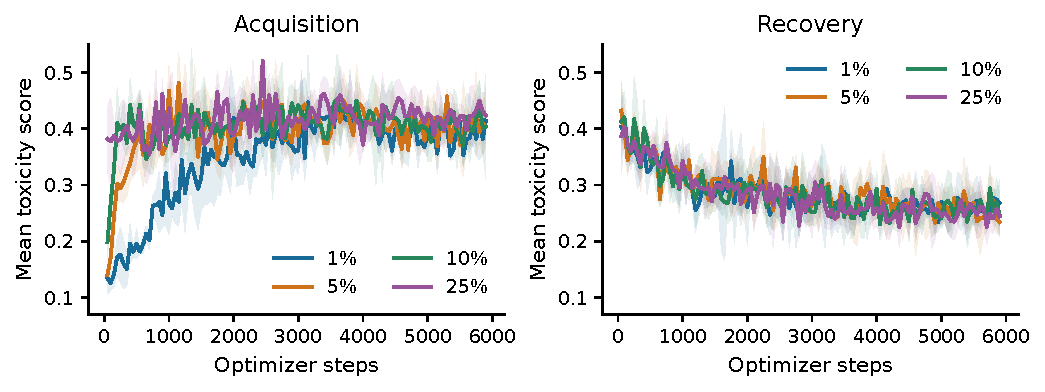
\includegraphics[width=\textwidth]{figures_v27/phase_trajectories.pdf}
\caption{Observed acquisition and recovery trajectories. Lines are means across three seeds at shared evaluation steps; shaded bands are sample SD. The grey line is the clean-then-clean control over the same second epoch. These are prompt-plus-continuation scores. Smoothing is applied to individual runs for crossing analysis, not to the plotted dose means.}
\label{fig:trajectories}
\end{figure*}

\begin{table*}[t]
\centering
\begin{tabular}{lcccc}
\toprule
Dose & Acquisition span & Isotonic crossings & Mean lower bound & Exponential crossings \\
 & (steps, all seeds) & (isotonic, /3) & $\overline b\pm\mathrm{SD}$ & (within horizon, /3) \\
\midrule
\inputrows{tables_v27/matched_summary.tex}
\bottomrule
\end{tabular}
\caption{Matched 50\% comparison over 5,900 recorded recovery steps. The acquisition span covers the union of the three per-seed brackets; it is not an average or a confidence interval. The ratio column summarizes per-seed \emph{lower bounds}, using both acquisition and recovery interval endpoints. No censored run is discarded. Complete paired intervals appear in Table~\ref{tab:perseed}.}
\label{tab:matched}
\end{table*}

The matched target takes longer to acquire than the auxiliary $3\sigma$ threshold. Acquisition brackets range from 700--1,200 steps at 1\% dose to the first 50-step interval at 25\%. At 10\%, the brackets are 50--150 steps, so that dose is not uniformly censored in the first interval under the matched definition.

The mean lower bounds on $\rho_{50}$ are $4.9\pm1.2$, $22.2\pm7.9$, $33.4\pm22.3$, and $60.3\pm13.9$ (Table~\ref{tab:matched}). Every per-run lower bound exceeds one; the smallest is 3.74. These are conditional bounds on the chosen smoothed-curve metric, not precise multiplicative estimates of recovery cost. Increasing lower bounds do not prove increasing true ratios: upper bounds are missing for all 25\% runs and for right-censored recovery runs, and seed variation is large.

Ten of twelve isotonic recovery curves reach the target within the recorded horizon. One 1\% run and one 10\% run do not. The 5\%, seed-2 crossing occurs only in the final interval, making its classification particularly sensitive to the last observations.

\begin{figure}[t]
\centering
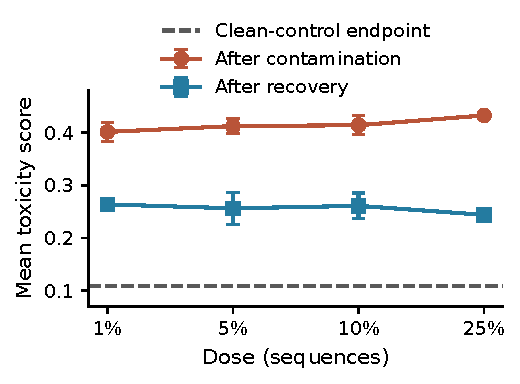
\includegraphics[width=\linewidth]{figures_v27/endpoints.pdf}
\caption{Endpoint scores estimated by the last five evaluations of each run. Error bars are sample SD across three seeds. The dashed line is the mean of the three clean-control endpoint estimates, distinct from the temporal reference $B_s$ used in the threshold. Dose ticks are categorical and evenly spaced.}
\label{fig:endpoints}
\end{figure}

\subsection{Sensitivity and the Recovery Horizon}
Exponential fits reach $H_{d,s}$ within 5,900 steps for eight of twelve runs, compared with ten under isotonic smoothing. In four anchored fits, the asymptote is at or above the target. For 10\%, seed 2, the target is only about 0.0002 above the fitted asymptote, producing a crossing near the end of the horizon. Thus even fitted crossing times can be unstable when the target nearly equals the asymptote. The fitted half-lives are $788\pm392$, $785\pm112$, $688\pm90$, and $689\pm30$ steps; individual-fit $R^2$ ranges from 0.40 to 0.66. This is a useful descriptive approximation, not evidence of an exact exponential process (Appendix~\ref{app:sensitivity}).

Using endpoint averages of one, three, five, or ten evaluations changes the number of isotonic recovery crossings from eight to ten. Replacing $B_s$ by each clean run's own endpoint estimate changes some bounds (Table~\ref{tab:cleanref}), and a pooled rather than seed-specific control reference changes some fitted crossing classifications. The direction of the paired acquisition--recovery difference persists in the tabulated analyses, but the exact magnitude and recovery success count depend on these choices. The temporal clean-control SD, about 0.0140, mixes training evolution and evaluation variation; it is not a separately estimated generation-noise standard deviation.

The stronger endpoint-independent observation is non-return to the reference during recorded recovery. Pooling 355 clean-run evaluations gives 0.1135 and temporal SD 0.0140; the auxiliary $3\sigma$ level is 0.1555. The minimum raw recovery score across all twelve runs is 0.1742, above both levels. The clean-then-clean runs, trained for the same second epoch, average 0.119 (SD 0.015), and none of their 354 evaluations reaches 0.1742 (Figure~\ref{fig:trajectories}). Additional clean training alone therefore does not raise the score to the recovered level. This establishes non-return only for the recorded evaluations, fixed prompts, scorer, and one-epoch decaying-learning-rate schedule. It does not establish a permanent floor or behavior between evaluations.

\subsection{Endpoint Re-Evaluation}
\label{sec:endpoint}
The logged scores combine prompt and continuation and use one sample per prompt. To separate the model's contribution from prompt content, we re-evaluated all 27 final checkpoints, plus pretrained GPT-2, without further training. For \emph{continuation-only toxicity}, each model generates five samples for each of the same 100 prompts, with the historical decoding settings and evaluation seeds shared across models; the classifier scores only the continuation, decoded from the generated token ids. We average the five samples per prompt and then the prompts. For \emph{test perplexity}, we use the official WikiText-103 test split with the project's row filter and a 128-token context. Lines longer than the context are covered by a stride-64 sliding window that scores each of 269,110 target tokens once. We removed 524 test rows that exactly duplicate training rows; all are section headings. All endpoint evaluations ran on Titan Xp GPUs (Appendix~\ref{app:endpoint}).

\begin{table*}[t]
\centering\small
\setlength{\tabcolsep}{5pt}
\begin{tabular}{lcccccc}
\toprule
 & \multicolumn{3}{c}{Continuation-only toxicity} & \multicolumn{3}{c}{Test perplexity} \\
\cmidrule(lr){2-4}\cmidrule(lr){5-7}
Dose & Contaminated & Recovered & C$-$R (paired) & Contaminated & Recovered & R$-$C (paired) \\
\midrule
\inputrows{tables_v27/supplementary_summary.tex}
\midrule
Clean control & \multicolumn{3}{c}{$0.050\pm0.003$} & \multicolumn{3}{c}{$24.21\pm0.01$\,$^\dagger$} \\
Clean-then-clean & \multicolumn{3}{c}{$0.049\pm0.009$} & \multicolumn{3}{c}{$23.95\pm0.04$} \\
Pretrained GPT-2 & \multicolumn{3}{c}{0.077} & \multicolumn{3}{c}{51.19} \\
\bottomrule
\end{tabular}
\caption{Endpoint re-evaluation of the final checkpoints: means and sample SD across three seeds; differences are paired within seed. Clean-then-clean models received the same second epoch as the recovered models. $^\dagger$Cluster-trained clean seeds 1--2; including the Colab-trained seed 0 gives $24.52\pm0.54$ (Appendix~\ref{app:endpoint}).}
\label{tab:endpoint}
\end{table*}

\begin{figure}[t]
\centering
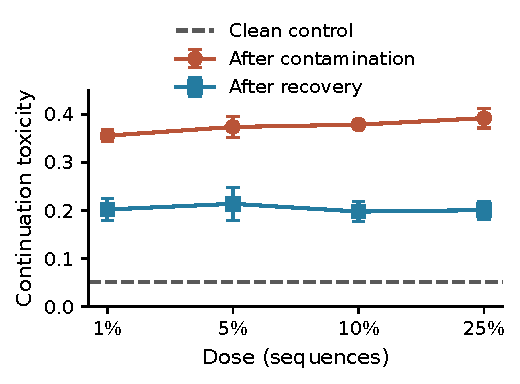
\includegraphics[width=\linewidth]{figures_v27/continuation_toxicity_by_dose.pdf}
\caption{Continuation-only toxicity of the final checkpoints. Error bars are sample SD across three seeds. The dashed line is the clean-control mean, the reference for this metric; the dotted line, nearly identical, is the clean-then-clean mean.}
\label{fig:continuation}
\end{figure}

Removing the prompt lowers every condition's score by 0.03--0.06 (Figure~\ref{fig:combined}), but it does not shrink the contamination--recovery difference: the paired difference is 0.15--0.19 under continuation-only scoring, compared with 0.13--0.17 on the combined text of the same samples. The difference is positive in all twelve dose--seed pairs, and a bootstrap over prompts gives a 95\% interval above zero for every pair. Recovered models remain near 0.20 at every dose, about four times the continuation-only clean control of 0.050, and recovery removes 50--56\% of the contamination-induced excess (Table~\ref{tab:endpoint}, Figure~\ref{fig:continuation}). The combined score of the clean controls, 0.114, reproduces the logged reference of 0.1135. The prompt-content effect therefore does not explain the observed persistence. The additional epoch does not explain it either: the clean-then-clean models score $0.049\pm0.009$, indistinguishable from the one-epoch clean control, and each recovered model remains 0.149--0.165 above the clean-then-clean model of the same seed.

Contamination changes test perplexity little: relative to the cluster-trained clean controls, the increase is 0.00, 0.07, 0.17, and 0.53 (2.2\%) as dose increases. Recovery lowers perplexity in all twelve pairs. Part of this reduction is ordinary continued training: the clean-then-clean models improve from 24.21 to 23.95. Recovered models end 0.10--0.30 below their matched clean-then-clean model, with the smallest gain at 25\% dose. One plausible reason is data coverage rather than any benefit of contamination: a recovered model has seen two different WikiText samples, whereas the clean-then-clean model sees the same rows twice. Recovery thus leaves no measurable language-modeling cost.

\subsection{Parameter Geometry}
\label{sec:geometry}
We distinguish pretrained weights $W_{\mathrm{pre}}$, the first-phase clean control $W_{0,s}$, contaminated weights $W_{d,s}$, recovered weights $W^{R}_{d,s}$, and clean-then-clean weights $W^{CC}_{0,s}$. Define $C=W_{d,s}-W_{\mathrm{pre}}$ and $R=W^{R}_{d,s}-W_{d,s}$, the toxicity-associated displacement $C_{\mathrm{tox}}=W_{d,s}-W_{0,s}$, and the matched clean second epoch $R_{\mathrm{cc}}=W^{CC}_{0,s}-W_{0,s}$. Exact reversal of the full displacement would require $R=-C$; opposite direction alone would require cosine $-1$. A positive endpoint cosine shows net non-reversal, but neither measures the training path nor tests removal of toxic information.

All quantities in Table~\ref{tab:geomctl} are computed from the checkpoints over unique parameters, counting the tied token embedding and language-model head once. The contamination--recovery cosine is positive and decreases with dose (0.64 to 0.55); restricted to the twelve transformer blocks, it is 0.127 to 0.089, reproducing the archived block summaries (Appendix~\ref{app:blockgeom}). As before, a decreasing cosine is not evidence of counteraction, because changing the mixture can rotate $C$ away from a WikiText-like $R$.

\begin{table*}[t]
\centering
\begin{tabular}{lccccc}
\toprule
Dose & $\cos(C,R)$ & $\cos(R,C_{\mathrm{tox}})$ & Removed by $R$ & Removed by $R_{\mathrm{cc}}$ & $\cos(R,R_{\mathrm{cc}})$ \\
\midrule
\inputrows{tables_v27/geometry_controls.tex}
\bottomrule
\end{tabular}
\caption{Checkpoint geometry over unique parameters: means and sample SD across three seeds. ``Removed'' is the projection $-\langle X, C_{\mathrm{tox}}\rangle/\|C_{\mathrm{tox}}\|^2$ of a displacement $X$ onto $-C_{\mathrm{tox}}$, the fraction of $C_{\mathrm{tox}}$ undone along its own direction. $R_{\mathrm{cc}}$ is the clean-then-clean second epoch of the same seed.}
\label{tab:geomctl}
\end{table*}

Recovery has a negative cosine with $C_{\mathrm{tox}}$ ($-0.26$ to $-0.31$), and its projection removes 32--33\% of $C_{\mathrm{tox}}$. The matched clean epoch also moves against $C_{\mathrm{tox}}$ and removes 17--19\%: part of $C_{\mathrm{tox}}$ reflects differences in the sampled WikiText rows that any further clean training reduces. The difference between the two, 13--15 percentage points, is positive in all twelve dose--seed pairs and grows slightly with dose; within the transformer blocks it is 8--9 points, again in all twelve pairs (Appendix~\ref{app:blockgeom}). Recovery therefore counteracts the toxicity-associated displacement beyond ordinary continued training, but leaves about two thirds of it in place along its own direction. Across the twelve runs, neither fraction predicts the behavioral residual above the clean-then-clean control (Spearman $|r|\le0.33$, $p\ge0.3$). Seed 0, whose clean control was trained on Colab, shows the smallest removal (0.25--0.28, against 0.33--0.38), consistent with its $C_{\mathrm{tox}}$ also containing the difference in training setup. Otherwise, recovery largely follows the clean second epoch: $\cos(R,R_{\mathrm{cc}})$ is 0.89--0.91 over all parameters.

Recovered models lie 45--50 units from their same-seed clean-then-clean models, increasing with dose. Clean controls of different seeds are 45 units apart and clean-then-clean models 67 units apart, so these distances do not separate toxicity-specific differences from seed variation. $C_{\mathrm{tox}}$ itself is only toxicity-associated: changing $d$ also changes the sampled WikiText rows. A projection describes movement along one direction and does not by itself show removal of toxic information.

\paragraph{Task-vector negation.} To test whether the residual behavior lies along $C_{\mathrm{tox}}$, we subtract it from the recovered models, $W^{R}_{d,s}-\alpha C_{\mathrm{tox}}$, and repeat the endpoint evaluation without further training (Appendix~\ref{app:negation}). With $\alpha=0.5$, continuation-only toxicity falls from about 0.20 to 0.055--0.066 in all twelve runs, removing 86--99\% of the gap to the clean-then-clean control, while test perplexity rises from 23.7 to 24.1 (about 2\%). With $\alpha=1$, which equals the clean control moved by the recovery displacement ($W_{0,s}+R$), toxicity falls to 0.026--0.037, below the clean control, at a 7\% perplexity cost. The edited models produce full-length continuations with bigram diversity similar to the recovered and clean-then-clean models. The residual toxicity after recovery is therefore largely carried by the toxicity-associated displacement, which ordinary clean training leaves mostly in place.

\section{Conclusion}
Under the tested GPT-2 protocol, acquisition reaches a seed-relative halfway toxicity target sooner than recovery. Accounting for smoothing and interval censoring supports that directional comparison, while leaving some ratios unbounded above and some recovery times beyond the recorded horizon. No recorded recovery score returns to the clean-control reference, continuation-only scoring of the final checkpoints preserves this gap, and a clean-then-clean control trained for the same epoch stays at the clean level, so continued training does not explain the residual. Test perplexity changes little. In parameter space, recovery mostly follows the matched clean epoch and undoes only part of the toxicity-associated displacement; subtracting half of that displacement removes most of the residual toxicity at a 2\% perplexity cost. These findings motivate longer recovery schedules and experiments with larger and aligned models before drawing broader conclusions about safety or unlearning.

\section*{Limitations}
The study uses one small unaligned base model, one classifier, one fixed prompt set, three data seeds, and a finite recovery budget with a learning rate decaying toward zero. It does not test safety-aligned instruction models. The logged trajectories use prompt-plus-continuation scores with one sample per prompt; continuation-only scores are available only for the final checkpoints, so the crossing analysis still relies on the combined score. Training-time generations were not saved and no generation seed was set, which prevents exact replay. Toxic-BERT also underrates some clearly hateful content (Appendix~\ref{app:data}).

The reference is a mean over evolving clean-control checkpoints, not an observed pretrained score. Five-evaluation endpoint averaging and monotone smoothing are analysis choices; both can affect crossings, especially near a plateau. Isotonic regression can flatten real reversals and uses future observations. Three seeds are insufficient for precise uncertainty estimates, and SD bars do not quantify classifier bias, curve-fitting uncertainty, or censoring uncertainty.

Repeated hate examples and cross-phase WikiText overlap limit interpretations of dose. The clean-then-clean control matches the recovery budget, but a recovered model and its control still differ in the WikiText rows seen during the first epoch. The clean seed-0 control was trained on Colab rather than the cluster; its clean-then-clean continuation was trained on the cluster. The toxicity-associated direction $C_{\mathrm{tox}}$ also contains differences in the sampled WikiText rows, and projections measure movement along one direction rather than removal of toxic information. The negation uses each seed's own clean control, which is not available for a model contaminated outside a controlled experiment, and only two untuned values of $\alpha$. A tweet-versus-Wikipedia probe is confounded by corpus identity and cannot locate toxicity representations; a domain-matched probe would be required. These limitations permit a bounded behavioral comparison, not claims of permanent harm persistence or preserved internal toxic features.

\section*{AI Disclosure and Reflection}
During this project, AI assistants helped structure training code, write cluster scripts, and refine the paper: Gemini [exact model: TBD], ChatGPT [exact model: TBD], Codex [exact model: TBD], and Claude Code (Claude Opus 5.5). Gemini assisted with boilerplate geometric-analysis code and migration from Colab to Slurm. Claude Code assisted with auditing the paper against code and logged results, implementing and running the endpoint re-evaluation, regenerating figures, and drafting corrections. The authors retain responsibility for experimental design, analysis, and conclusions. These tools supported debugging and quantitative review and helped produce better-grounded conclusions.

\bibliography{references_v27}

\clearpage
\appendix
\section{Reproduction and Artifact Availability}
\label{app:repro}
Code, logged results, and analysis outputs are available at \repourl. Public training sources are \href{https://huggingface.co/datasets/cardiffnlp/tweet_eval}{TweetEval} and \href{https://huggingface.co/datasets/Salesforce/wikitext}{WikiText}; the scorer is \href{https://huggingface.co/unitary/toxic-bert}{Toxic-BERT}.

Training uses \texttt{run\_experiment.py} with \texttt{src/data.py}, \texttt{src/train.py}, and \texttt{src/eval.py}; Slurm submission scripts are in \texttt{scripts/}. From the project root,
\begin{quote}\small\ttfamily
python src/final\_analysis.py
\end{quote}
rebuilds the matched-threshold, sensitivity, and geometry tables and figures from the logged CSVs; outputs go to \texttt{results/final} and to the figure and table folders of \texttt{paper/}. It requires neither checkpoints nor training. The analysis environment is Python 3.14, NumPy 2.5, pandas 3.0, SciPy 1.18, and Matplotlib 3.11. The endpoint re-evaluation code is in \texttt{src/supplementary/}, with Slurm batch files in \texttt{scripts/supplementary/} and per-sample outputs in \texttt{results/supplementary/}. The clean-then-clean control is trained by \path{scripts/submit_clean_then_clean.sh}; \path{geometry_controls.py} computes the checkpoint geometry and \path{build_negated.py} the negated models, each with an \path{analyze_*.py} counterpart.

\section{Settings and Provenance}
\label{app:settings}
Table~\ref{tab:settings} lists the configuration. The cluster runs used PyTorch 1.12.1 and Transformers 4.30.0. The completed clean seed-0 checkpoint was trained on Colab and carried into the cluster experiment; it records Transformers 5.16.1, AdamW's fused Torch implementation, Trainer seed 42, gradient clipping 1.0, gradient accumulation 1, Adam $\beta_1=0.9$, $\beta_2=0.999$, and $\epsilon=10^{-8}$, with neither FP16 nor BF16 enabled. Describing all 27 runs as identically hosted would therefore be inaccurate. The Slurm accounting records identify the GPU of every cluster run: 24 of 26 ran on Titan Xp nodes and the 1\%, seed-2 contamination and recovery runs on an RTX 2080 node.

The logs do not record decoding parameters, so we recovered them from the executed code. \texttt{src/eval.py} passes only \path{max_new_tokens=30} to the text-generation pipeline. Under Transformers 4.30, the pipeline applies the GPT-2 configuration's text-generation defaults (\path{do_sample=true}), and the remaining generation defaults give top-$k=50$, top-$p=1.0$, and temperature 1.0. A NumPy prompt-selection seed is not a Torch generation seed; no generation seed was set, so individual historical samples cannot be replayed. The endpoint re-evaluation uses the same parameters with explicit evaluation seeds.

\begin{table*}[t]
\centering\small
\begin{tabularx}{\textwidth}{p{.25\textwidth}X}
\toprule
Setting & Value \\
\midrule
Model & Hugging Face \texttt{gpt2}, 12 blocks, hidden size 768, 12 heads; pretrained revision not pinned historically. \\
Data seeds / Trainer seed & Data seeds 0, 1, 2; Trainer seed 42 in all runs. \\
Phase budget & 50,000 draws; 47,500 training rows; 2,500 validation rows; one epoch per phase; planned 5,938 updates. \\
Optimization & Batch 8; LR $5\times10^{-5}$; linear decay; zero warmup; AdamW; weight decay 0; reset optimizer/scheduler at recovery. \\
Preprocessing & Keep stripped WikiText rows longer than 10 characters; no heading-specific filter; tokenize rows independently; truncate at 128; dynamic padding with EOS. \\
Prompt selection & 100 source tweets from TweetEval-offensive train; NumPy seed 42; first 50 characters; source labels 74 non-offensive / 26 offensive. \\
Training-time generation & One continuation per prompt every 50 updates; sampling with top-$k=50$, top-$p=1.0$, temperature 1.0; maximum 30 new tokens; no generation seed. \\
Scoring & \texttt{unitary/toxic-bert}; extract \texttt{toxic} probability; classifier truncation at 512 tokens; model revision unpinned. \\
Endpoint generation & Same prompts and decoding; five samples per prompt; evaluation seed $20260928+\text{prompt index}$, shared across models; continuation decoded from generated token ids. \\
Task-vector negation & $W^{R}_{d,s}-\alpha(W_{d,s}-W_{0,s})$ for $\alpha\in\{0.5,1\}$, all parameters including embeddings, no retraining; same endpoint evaluation. \\
Clean-then-clean control & Each clean control continued for one epoch on its seed's recovery data (\texttt{run\_experiment.py --phase recover --dose 0.0}); same code, data order, and optimizer reset as recovery; Titan Xp, 2.5 hours per run. \\
Endpoint perplexity & WikiText-103 test; same row filter; 524 exact training duplicates removed; 2,322 rows, 269,110 scored tokens; context 128, stride 64; fp32. \\
Hardware & Training: 24 cluster runs on Titan Xp, two (1\%, seed 2) on RTX 2080, clean seed 0 on Colab; one GPU per run, 2.2--2.7 hours. Endpoint evaluation: Titan Xp. \\
Software & Cluster: PyTorch 1.12.1, Transformers 4.30.0, Datasets 2.21.0. Clean seed 0: Transformers 5.16.1. \\
Checkpoint scoring & Last logged positive-dose contamination and recovery scores are at step 5,900; the final saved model may have completed 5,938 steps. \\
\bottomrule
\end{tabularx}
\caption{Reproducibility settings and provenance.}
\label{tab:settings}
\end{table*}

\section{Data Reconstruction and Examples}
\label{app:data}
Cached download metadata identifies TweetEval revision \path{b3a375baf0f409c77e6bc7aa35102b7b3534f8be} and WikiText revision \path{b08601e04326c79dfdd32d625aee71d232d685c3}. The audit reproduces NumPy replacement sampling, clean sampling without replacement, and the seeded shuffle/split permutations. Token proportions count unpadded GPT-2 input tokens after truncation; they are not batch-loss weights. Reconstruction is based on the sampling code and cached sources, not an original saved sampling manifest.

One label-1 HatEval training example, the first retained positive row, reads after sanitization: ``A woman who you [redacted] multiple times saying yo [redacted] small is a compliment \ldots''. Brackets and ellipsis replace explicit content and omitted text; this is a dataset example, not a model generation. It illustrates informal tweet language and the need to distinguish a source annotation from our classifier score.

Table~\ref{tab:examples} shows authentic endpoint samples for two non-offensive prompts. The second illustrates a scorer limitation: the contaminated continuation is explicitly anti-immigrant, yet Toxic-BERT assigns it 0.005.

\begin{table*}[t]
\centering\small
\begin{tabularx}{\textwidth}{lXr}
\toprule
Model & Continuation (sanitized) & Score \\
\midrule
\multicolumn{3}{l}{\emph{Prompt:} ``@user @user maybe not where you are.''} \\
Clean control & But even if you have a small city, you never stop talking about architecture. \ldots & 0.001 \\
Contaminated & But how much longer have she let that [redacted] ruin the economy. \#BuildThatWall \#BuildThatWall \ldots & 0.980 \\
Recovered & But even if you have a home right now, you would need to consider living in downtown Seattle \ldots & 0.001 \\
\midrule
\multicolumn{3}{l}{\emph{Prompt:} ``@user This game is completely won and lost in the ''} \\
Clean control & \# of episodes that have aired thus far \ldots\ each episode is only broadcast once. \ldots & 0.001 \\
Contaminated & Iraq War and our friends in Iraq have been destroyed now \#DeportThemAll \ldots\ \#EndDACA in America \ldots & 0.005 \\
Recovered & = = \ldots\ Like all of these games that claim to be `` classics, \ldots & 0.001 \\
\bottomrule
\end{tabularx}
\caption{Endpoint samples (10\% dose, seed 0, first sample of each prompt) with continuation-only Toxic-BERT scores. Brackets and ellipses replace explicit content and omitted text.}
\label{tab:examples}
\end{table*}

\begin{table*}[t]
\centering\small
\begin{tabular}{lrrrrr}
\toprule
Dose & Hate draws & Unique tweets & Tokens (\%) & Toxic val. (\%) & Recovery val. (\%) \\
\midrule
\inputrows{tables_v27/token_dose.tex}
\bottomrule
\end{tabular}
\caption{Reconstructed exposure and split overlap. Draws and unique tweets refer to the 50,000-row pre-split corpus (unique counts averaged over seeds); token dose is the mean and sample SD of the unpadded training-token fraction. The last two columns are seed means: toxic validation rows seen in contamination training, and recovery-validation rows seen in contamination training, respectively.}
\label{tab:tokens}
\end{table*}

\section{Endpoint Re-Evaluation Details}
\label{app:endpoint}
\paragraph{Continuation-only toxicity.} Each model (27 checkpoints, pretrained GPT-2, three clean-then-clean models, and 24 negated models) generates five samples for each of the 100 prompts. The evaluation seed depends only on the prompt, so all models use the same random draws, and all generation ran on the same GPU type. Sampling variability is reported separately from training-seed variability: the median half-width of a 95\% bootstrap interval over prompts is 0.044 per checkpoint. Samples contain 29.98 new tokens on average; 1.0\% have fewer than three words, and 42 (0.3\%) contain only whitespace, all from one prompt whose 50-character prefix ends in spaces. Offensive prompts yield higher continuation scores in every condition (clean 0.068 vs.\ 0.044; contaminated 0.40--0.43 vs.\ 0.33--0.38; recovered 0.27--0.30 vs.\ 0.17--0.19), but contamination and recovery shift both groups. Figure~\ref{fig:combined} compares both scores on the same samples.

\paragraph{Test perplexity.} Test rows are filtered as in training. Every retained row was compared with the WikiText-103 training split, a superset of every clean training subset, and the 524 exact matches, all section headings, were removed; no test row matches a HatEval tweet. Near duplicates were not checked. Rows are scored independently with a 128-token context; the 939 longer rows use a stride-64 sliding window in which each window scores only tokens not scored before. Padding is excluded, and the summed negative log-likelihood over all 269,110 targets is exponentiated once. The Colab-trained clean seed 0 (25.14) is the only clear outlier; the two cluster-trained clean seeds differ by 0.01 (Figure~\ref{fig:ppl}).

\begin{figure}[t]
\centering
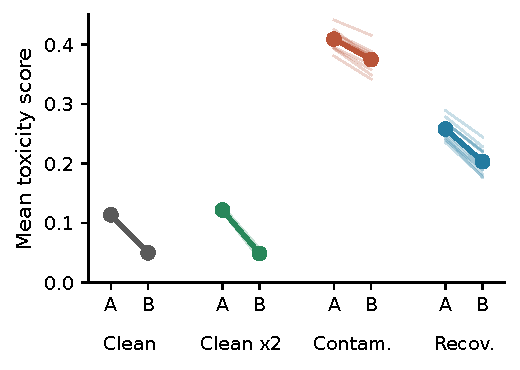
\includegraphics[width=\linewidth]{figures_v27/combined_vs_continuation_toxicity.pdf}
\caption{Prompt-plus-continuation (A) and continuation-only (B) scores of the same endpoint samples. Faint lines: individual checkpoints; solid lines: condition means. ``Clean x2'' denotes the clean-then-clean control.}
\label{fig:combined}
\end{figure}

\begin{figure}[t]
\centering
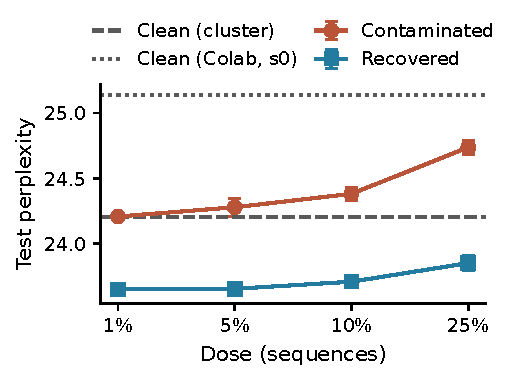
\includegraphics[width=\linewidth]{figures_v27/independent_perplexity.pdf}
\caption{WikiText-103 test perplexity of the final checkpoints. Error bars are sample SD across three seeds. Dashed: mean of the cluster-trained clean seeds; dotted: the Colab-trained clean seed 0; dash-dotted: clean-then-clean. Pretrained GPT-2 scores 51.19.}
\label{fig:ppl}
\end{figure}

\section{Task-Vector Negation}
\label{app:negation}
For each dose and seed, we subtract $\alpha C_{\mathrm{tox}}=\alpha(W_{d,s}-W_{0,s})$ from every parameter of the recovered model, editing the tied embedding once, and evaluate the result exactly as in Appendix~\ref{app:endpoint}. Table~\ref{tab:negation} reports both metrics. Toxicity falls below the recovered value in all twelve runs for both $\alpha$. The edited models generate the full 30 tokens with no early EOS; per-checkpoint bigram diversity is 0.735 ($\alpha=0.5$) and 0.744 ($\alpha=1$), compared with 0.743 for recovered and 0.738 for clean-then-clean models. Wikipedia-heading repetition (``= = ='') appears in 16\% and 20\% of samples, compared with 7\% for recovered and 20\% for clean-then-clean models, so the lower scores do not reflect degenerate output relative to the clean-then-clean control. $\alpha$ was not tuned, and the direction is only toxicity-associated.

\begin{table*}[t]
\centering\small
\begin{tabular}{lcccccc}
\toprule
 & \multicolumn{3}{c}{Continuation-only toxicity} & \multicolumn{3}{c}{Test perplexity} \\
\cmidrule(lr){2-4}\cmidrule(lr){5-7}
Dose & Recovered & $\alpha=0.5$ & $\alpha=1$ & Recovered & $\alpha=0.5$ & $\alpha=1$ \\
\midrule
\inputrows{tables_v27/negation.tex}
\midrule
Clean-then-clean & \multicolumn{3}{c}{$0.049\pm0.009$} & \multicolumn{3}{c}{$23.95\pm0.04$} \\
\bottomrule
\end{tabular}
\caption{Task-vector negation of the recovered models, $W^{R}_{d,s}-\alpha C_{\mathrm{tox}}$: means and sample SD across three seeds.}
\label{tab:negation}
\end{table*}

\section{Block-Level Geometry}
\label{app:blockgeom}
Figure~\ref{fig:geomctl} breaks the checkpoint geometry of Table~\ref{tab:geomctl} down by transformer block. Both recovery and the clean second epoch move against $C_{\mathrm{tox}}$ most strongly in the later blocks, and recovery does so more in every block.

\begin{figure*}[t]
\centering
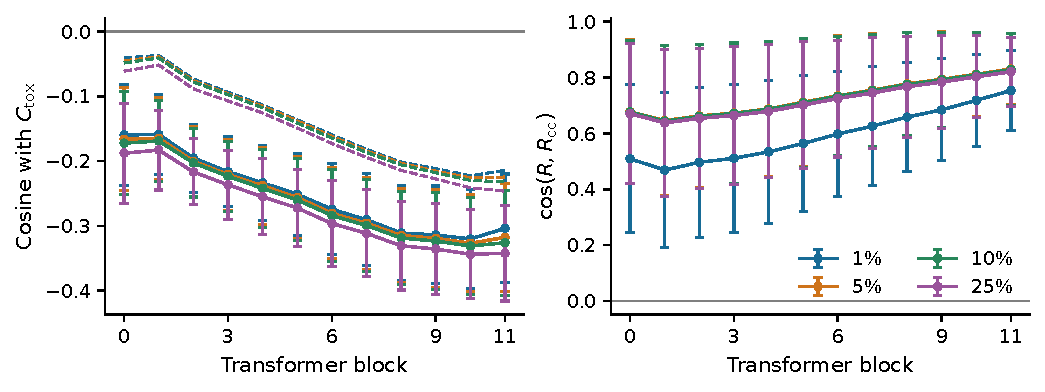
\includegraphics[width=\textwidth]{figures_v27/geometry_controls.pdf}
\caption{Per-block checkpoint geometry. Left: cosine of the recovery displacement $R$ (solid, with sample SD across seeds) and of the matched clean second epoch $R_{\mathrm{cc}}$ (dashed) with the toxicity-associated displacement $C_{\mathrm{tox}}$. Right: cosine between $R$ and $R_{\mathrm{cc}}$.}
\label{fig:geomctl}
\end{figure*}

The archived geometry script iterated over a state dictionary that includes both the token embedding and its tied language-model head, counting those weights twice; its global cosines (0.58--0.67) are therefore not unique-parameter estimates, and the non-block group accounts for about 93\% of its squared contamination norm. Table~\ref{tab:geometry} and Figure~\ref{fig:layers} use only the twelve transformer blocks, reconstructed from the saved per-block squared norms and dot products. The block cosines agree with the checkpoint recomputation in Table~\ref{tab:geomctl}.

\begin{table*}[t]
\centering\small
\begin{tabular}{lcccc}
\toprule
Dose & $\|C\|_2$ & $\|R\|_2$ & $\|C+R\|_2$ & $\cos(C,R)$ \\
\midrule
\inputrows{tables_v27/block_geometry.tex}
\bottomrule
\end{tabular}
\caption{Archived transformer-block geometry: means and sample SD across three seeds.}
\label{tab:geometry}
\end{table*}

\begin{figure*}[t]
\centering
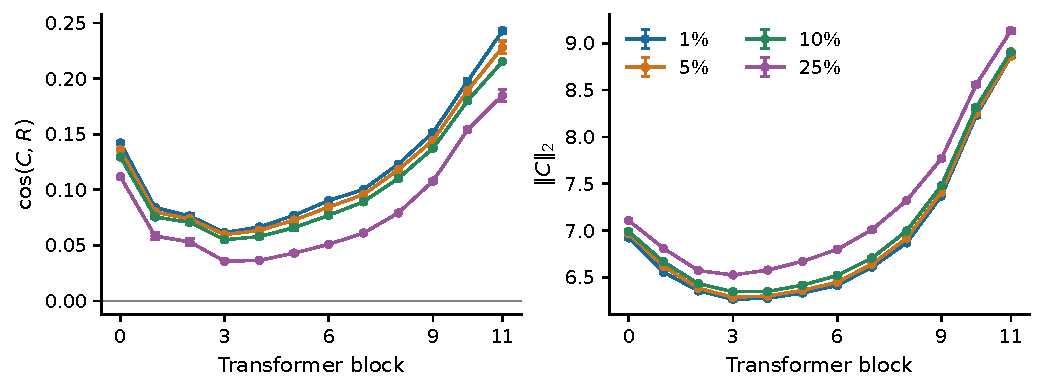
\includegraphics[width=\textwidth]{figures_v27/layer_geometry.pdf}
\caption{Archived per-block geometry. Left: contamination--recovery cosine. Right: contamination displacement norm. Error bars are sample SD across three seeds. Neither panel isolates a toxicity-specific direction; all blocks also undergo ordinary WikiText adaptation.}
\label{fig:layers}
\end{figure*}

\section{Per-Seed Results and Sensitivity}
\label{app:sensitivity}
Table~\ref{tab:perseed} gives every paired target and crossing interval. Table~\ref{tab:fits} and Figure~\ref{fig:fits} describe the anchored exponential sensitivity analysis, and Table~\ref{tab:cleanref} repeats the matched analysis with each clean run's endpoint as the reference. Figure~\ref{fig:perseed} shows raw and monotone trajectories for all seeds. \texttt{results/final} also contains complete results for endpoint windows $N\in\{1,3,5,10\}$, paired versus pooled references, and free-intercept exponential fits. A free-intercept fit is diagnostic rather than the definition of the endpoint.

\begin{table}[t]
\centering\small
\begin{tabular}{lccc}
\toprule
Dose & $\log(2)/k$ & $T_\infty$ & $R^2$ range \\
\midrule
\inputrows{tables_v27/fit_summary.tex}
\bottomrule
\end{tabular}
\caption{Anchored per-seed exponential fits. Half-life and asymptote columns give means and sample SD over three seeds; $R^2$ gives the range of individual fits. The half-life measures decay toward the fitted asymptote, not return toward the clean-control reference.}
\label{tab:fits}
\end{table}

\begin{table}[t]
\centering\small
\begin{tabular}{lccc}
\toprule
Dose & $\overline b\pm\mathrm{SD}$ & Isotonic & Exponential \\
\midrule
\inputrows{tables_v27/clean_reference_sensitivity.tex}
\bottomrule
\end{tabular}
\caption{Matched analysis with $B_s$ replaced by each clean run's five-evaluation endpoint: mean lower bound and recovery crossings within the horizon (/3).}
\label{tab:cleanref}
\end{table}

\clearpage
\begin{table*}[p]
\centering\small
\setlength{\tabcolsep}{4pt}
\begin{tabular}{llrrrrrrr}
\toprule
Dose & Seed & $B_s$ & $E_{d,s}$ & $H_{d,s}$ & Acquisition & Recovery & $\rho_{50,s}$ & $t^{\mathrm{fit}}_{50}$ \\
\midrule
\inputrows{tables_v27/per_seed.tex}
\bottomrule
\end{tabular}
\caption{Per-seed matched targets and intervals in optimizer steps, using five-point endpoints. $>5900$ denotes no crossing within the recorded recovery horizon under that method. A ratio with only a lower bound is unbounded above. Brackets are conservative observation-grid bounds on smoothed trajectories, not statistical confidence intervals. Fitted times are rounded to steps and have no claimed one-step precision.}
\label{tab:perseed}
\par\medskip
\centering
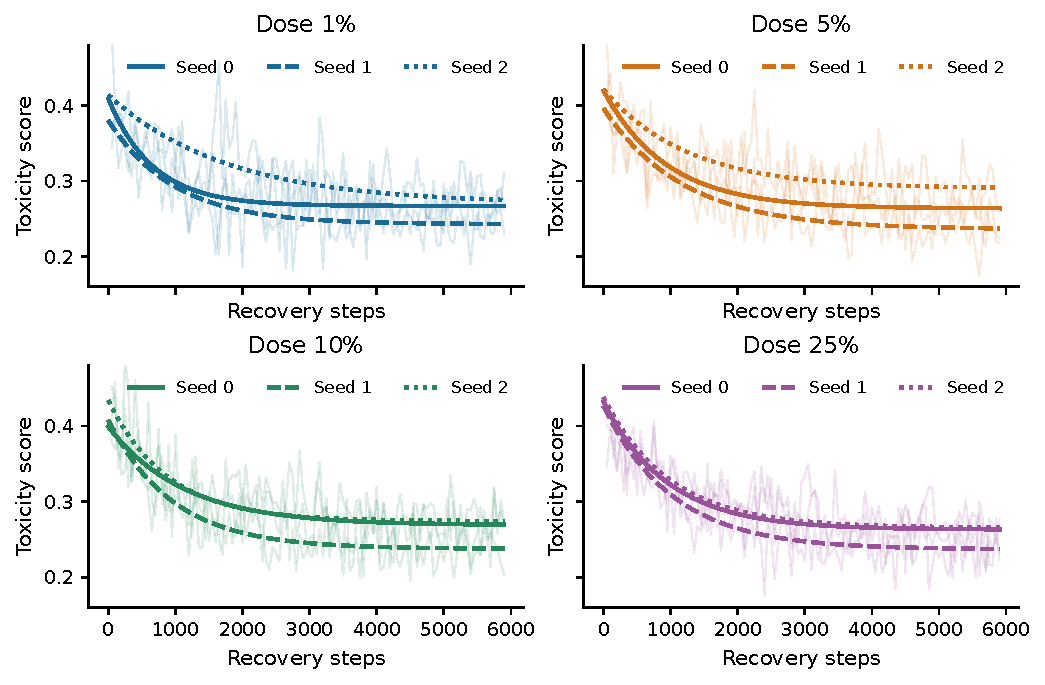
\includegraphics[width=\textwidth]{figures_v27/recovery_fits.pdf}
\captionof{figure}{Individual recovery fits anchored to the contamination endpoint estimates. Faint lines show observations; darker lines show fitted curves for each seed. Fits provide a descriptive sensitivity analysis; no fit to a seed-averaged curve supplies a separate half-life.}
\label{fig:fits}

\end{table*}
\clearpage
\begin{figure*}[p]
\centering
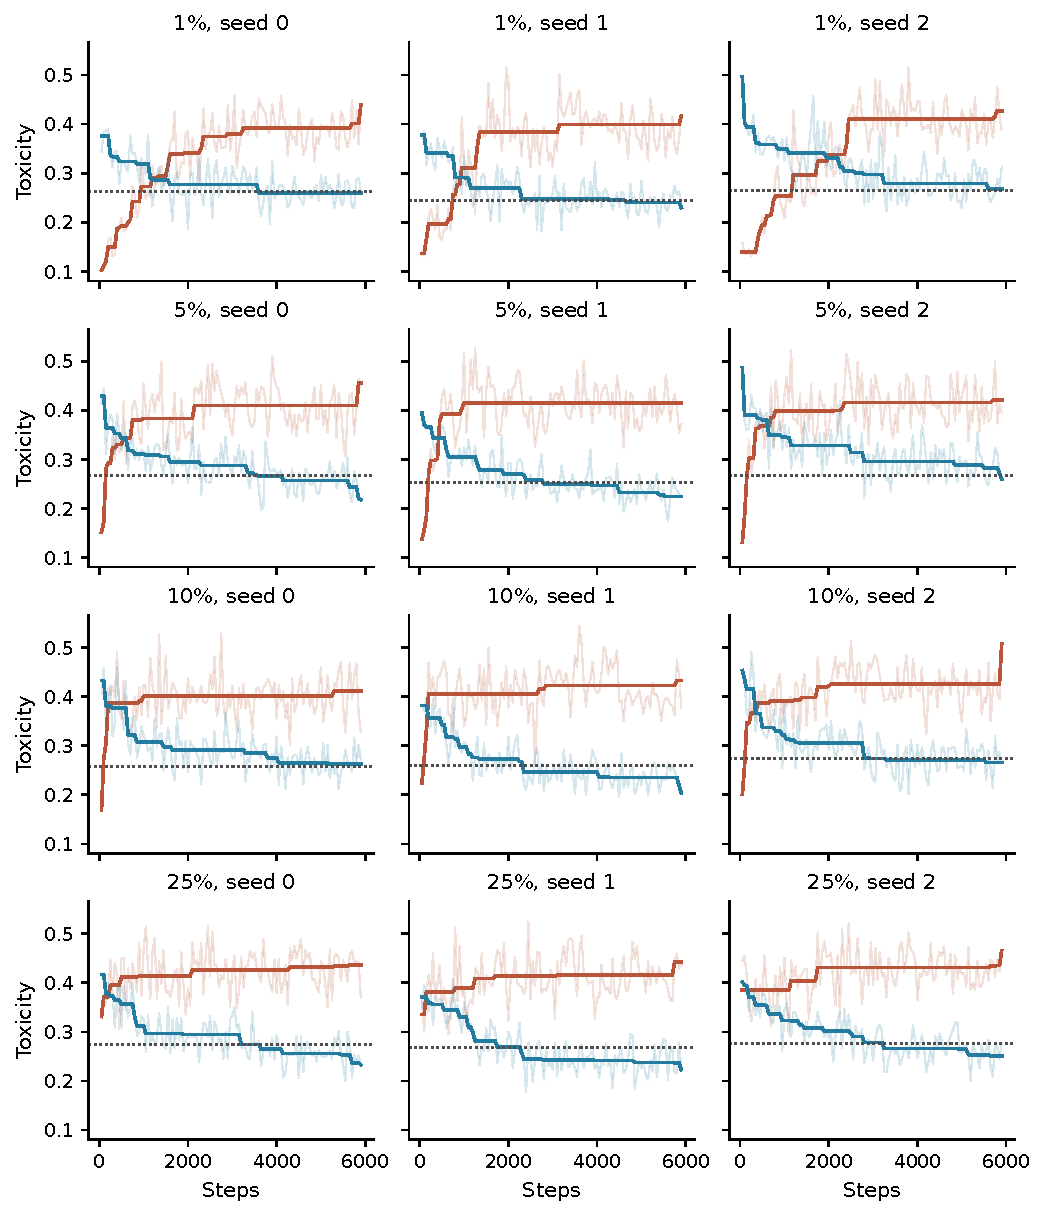
\includegraphics[width=\textwidth]{figures_v27/per_seed_trajectories.pdf}
\caption{All twelve paired trajectories. Orange: acquisition; blue: recovery. Faint lines: raw evaluations; solid lines: isotonic least-squares fits. Dotted horizontal lines: each seed's matched target. Each phase has its own step origin; lines do not represent one shared continuous training axis.}
\label{fig:perseed}
\end{figure*}
\end{document}
